\chapter[Planteamientos]{Planteamientos}
% \label{cp:introduction}

{
\parindent0pt

\vspace{.935em}

\section{Problema 1 (40\%)}
Con base en la arquitectura definida en la Figura, modelar un conjunto de reglas vía NetFilter/IPTables, así:


\begin{figure}
    \centering
    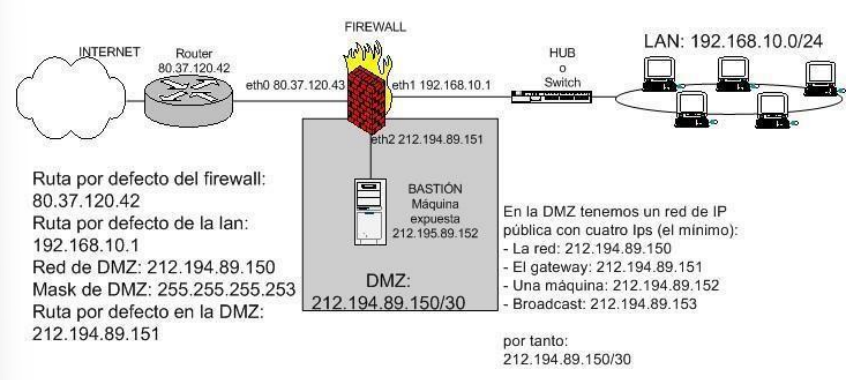
\includegraphics[width=0.5\linewidth]{topologia.png}
    \caption{Topología de red}
    \label{fig:arquitectura-de-red}
\end{figure}


\subsection{Análisis de la Arquitectura de Red}

Analizando la arquitectura mostrada, parece que se presenta la topología clásica de \textbf{defensa en profundidad} con las tres zonas de seguridad claramente diferenciadas:

\begin{itemize}
    \item \textbf{Internet (Zona no confiable):} IP pública del router: 80.37.120.42
    \item \textbf{DMZ (Zona semi-confiable):} Red 212.194.89.150/30
    \begin{itemize}
        \item Gateway: 212.194.89.151 (interfaz eth2 del firewall)
        \item Servidor expuesto: 212.194.89.152
        \item Broadcast: 212.194.89.153
    \end{itemize}
    \item \textbf{LAN Interna (Zona confiable):} Red 192.168.10.0/24
    \begin{itemize}
        \item Gateway: 192.168.10.1 (interfaz eth1 del firewall)
    \end{itemize}
\end{itemize}

\textbf{Interfaces del Firewall:}
\begin{itemize}
    \item \texttt{eth0}: 80.37.120.43 (interfaz externa hacia Internet)
    \item \texttt{eth1}: 192.168.10.1 (interfaz interna hacia LAN)
    \item \texttt{eth2}: 212.194.89.151 (interfaz DMZ)
\end{itemize}



\subsection{Literal a}

\textbf{Permitir el tráfico de los clientes LAN a los Web Servers de la DMZ (*.151, *.152):}

% \subsubsection{Literal A: Permitir tráfico LAN → DMZ (Web Servers)}

Para permitir el acceso desde la red LAN hacia los servidores web en la DMZ, implementamos las siguientes reglas:

\begin{lstlisting}[language=bash, caption=Reglas para tráfico LAN hacia DMZ]
# Permitir HTTP (puerto 80) desde LAN hacia servidor DMZ .151
iptables -A FORWARD -s 192.168.10.0/24 -d 212.194.89.151 \
         -p tcp --dport 80 -m state --state NEW,ESTABLISHED -j ACCEPT

# Permitir HTTP (puerto 80) desde LAN hacia servidor DMZ .152
iptables -A FORWARD -s 192.168.10.0/24 -d 212.194.89.152 \
         -p tcp --dport 80 -m state --state NEW,ESTABLISHED -j ACCEPT

# Permitir HTTPS (puerto 443) desde LAN hacia servidor DMZ .151
iptables -A FORWARD -s 192.168.10.0/24 -d 212.194.89.151 \
         -p tcp --dport 443 -m state --state NEW,ESTABLISHED -j ACCEPT

# Permitir HTTPS (puerto 443) desde LAN hacia servidor DMZ .152
iptables -A FORWARD -s 192.168.10.0/24 -d 212.194.89.152 \
         -p tcp --dport 443 -m state --state NEW,ESTABLISHED -j ACCEPT

# Permitir DNS TCP desde LAN hacia servidores DMZ
iptables -A FORWARD -s 192.168.10.0/24 -d 212.194.89.151 \
         -p tcp --dport 53 -m state --state NEW,ESTABLISHED -j ACCEPT
iptables -A FORWARD -s 192.168.10.0/24 -d 212.194.89.152 \
         -p tcp --dport 53 -m state --state NEW,ESTABLISHED -j ACCEPT

# Permitir DNS UDP desde LAN hacia servidores DMZ
iptables -A FORWARD -s 192.168.10.0/24 -d 212.194.89.151 \
         -p udp --dport 53 -m state --state NEW,ESTABLISHED -j ACCEPT
iptables -A FORWARD -s 192.168.10.0/24 -d 212.194.89.152 \
         -p udp --dport 53 -m state --state NEW,ESTABLISHED -j ACCEPT
\end{lstlisting}

\textbf{Justificación técnica:}
\begin{itemize}
    \item Utilizamos el módulo \texttt{state} con \texttt{NEW,ESTABLISHED} para permitir conexiones nuevas y establecidas.
    \item Se incluyen tanto HTTP (80) como HTTPS (443) para soportar tráfico web seguro.
    \item DNS (53) se permite en TCP y UDP para resolución de nombres completa.
    \item Las reglas son específicas por dirección IP de destino para mayor control.
\end{itemize}

\subsection{Literal b}
\textbf{Permitir el tráfico desde Internet hacia los servidores de la DMZ WWW \& email Server}

% \subsubsection{Literal B: Permitir tráfico Internet → DMZ (WWW \& Email)}

Para exponer los servicios públicos de la DMZ a Internet:

\begin{lstlisting}[language=bash, caption=Reglas para servicios públicos en DMZ]
# === SERVICIOS WEB ===
# Permitir HTTP desde Internet hacia ambos servidores web DMZ
iptables -A FORWARD -i eth0 -d 212.194.89.151 \
         -p tcp --dport 80 -m state --state NEW,ESTABLISHED -j ACCEPT
iptables -A FORWARD -i eth0 -d 212.194.89.152 \
         -p tcp --dport 80 -m state --state NEW,ESTABLISHED -j ACCEPT

# Permitir HTTPS desde Internet hacia ambos servidores web DMZ
iptables -A FORWARD -i eth0 -d 212.194.89.151 \
         -p tcp --dport 443 -m state --state NEW,ESTABLISHED -j ACCEPT
iptables -A FORWARD -i eth0 -d 212.194.89.152 \
         -p tcp --dport 443 -m state --state NEW,ESTABLISHED -j ACCEPT

# === SERVICIOS DE EMAIL (asumiendo .152 como servidor de correo) ===
# SMTP estándar (puerto 25)
iptables -A FORWARD -i eth0 -d 212.194.89.152 \
         -p tcp --dport 25 -m state --state NEW,ESTABLISHED -j ACCEPT

# SMTP seguro - SMTPS (puerto 465)
iptables -A FORWARD -i eth0 -d 212.194.89.152 \
         -p tcp --dport 465 -m state --state NEW,ESTABLISHED -j ACCEPT

# SMTP con STARTTLS (puerto 587)
iptables -A FORWARD -i eth0 -d 212.194.89.152 \
         -p tcp --dport 587 -m state --state NEW,ESTABLISHED -j ACCEPT

# IMAP (puerto 143) e IMAPS (puerto 993)
iptables -A FORWARD -i eth0 -d 212.194.89.152 \
         -p tcp --dport 143 -m state --state NEW,ESTABLISHED -j ACCEPT
iptables -A FORWARD -i eth0 -d 212.194.89.152 \
         -p tcp --dport 993 -m state --state NEW,ESTABLISHED -j ACCEPT

# POP3 (puerto 110) y POP3S (puerto 995)
iptables -A FORWARD -i eth0 -d 212.194.89.152 \
         -p tcp --dport 110 -m state --state NEW,ESTABLISHED -j ACCEPT
iptables -A FORWARD -i eth0 -d 212.194.89.152 \
         -p tcp --dport 995 -m state --state NEW,ESTABLISHED -j ACCEPT
\end{lstlisting}

\textbf{Justificación técnica:}
\begin{itemize}
    \item Se especifica la interfaz de entrada \texttt{-i eth0} para asegurar que el tráfico provenga de Internet.
    \item Se incluyen todos los protocolos de correo estándar (SMTP, IMAP, POP3) y sus versiones seguras.
    \item Las reglas utilizan el módulo de estado para mantener el seguimiento de conexiones.
\end{itemize}


\subsection{Literal c}
\textbf{Proteger el Router de la DMZ y de la LAN para tráfico ICMP y Telnet:}

% \subsection{Literal C: Proteger el Router de la DMZ y LAN (ICMP y Telnet)}

Para proteger el router de accesos no autorizados:

\begin{lstlisting}[language=bash, caption=Reglas de protección del router]
# === BLOQUEO DE TELNET ===
# Bloquear Telnet desde DMZ hacia el router
iptables -A FORWARD -s 212.194.89.150/30 -d 80.37.120.42 \
         -p tcp --dport 23 -j DROP

# Bloquear Telnet desde LAN hacia el router
iptables -A FORWARD -s 192.168.10.0/24 -d 80.37.120.42 \
         -p tcp --dport 23 -j DROP

# === PROTECCIÓN ICMP ===
# Limitar ICMP echo-request (ping) desde DMZ - Anti-DoS
iptables -A FORWARD -s 212.194.89.150/30 -d 80.37.120.42 \
         -p icmp --icmp-type echo-request \
         -m limit --limit 1/s --limit-burst 3 -j ACCEPT

# Limitar ICMP echo-request (ping) desde LAN - Anti-DoS
iptables -A FORWARD -s 192.168.10.0/24 -d 80.37.120.42 \
         -p icmp --icmp-type echo-request \
         -m limit --limit 1/s --limit-burst 3 -j ACCEPT

# Permitir ICMP echo-reply desde DMZ
iptables -A FORWARD -s 212.194.89.150/30 -d 80.37.120.42 \
         -p icmp --icmp-type echo-reply -j ACCEPT

# Permitir ICMP echo-reply desde LAN
iptables -A FORWARD -s 192.168.10.0/24 -d 80.37.120.42 \
         -p icmp --icmp-type echo-reply -j ACCEPT

# Bloquear todos los demás tipos de ICMP hacia el router
iptables -A FORWARD -d 80.37.120.42 -p icmp -j DROP

# === LOGGING PARA ANÁLISIS FORENSE ===
# Registrar intentos de Telnet bloqueados
iptables -A FORWARD -d 80.37.120.42 -p tcp --dport 23 \
         -j LOG --log-prefix "TELNET_BLOCKED_TO_ROUTER: " \
         --log-level 4
\end{lstlisting}

\textbf{Justificación técnica:}
\begin{itemize}
    \item \textbf{Bloqueo de Telnet:} Se deniega completamente el acceso Telnet (puerto 23) por ser un protocolo inseguro.
    \item \textbf{Limitación ICMP:} Se implementa rate limiting (1 ping/segundo) para prevenir ataques DoS.
    \item \textbf{Logging:} Se registran intentos de acceso no autorizado para análisis posterior.
\end{itemize}



\subsection{Literal d}

\textbf{Precisar semánticamente una regla en de Detección de Intrusiones (basada en Snort) que permita alertar intentos de elevar privilegios ( “sudo -i” ) a cualquier servidor de la DMZ:}

% \subsection{Literal D: Regla Snort para Detección de Elevación de Privilegios}

\subsubsection{Regla Principal}

\begin{lstlisting}[language=snort, caption=Regla Snort para detectar sudo -i]
# Regla principal para detectar "sudo -i" en tráfico hacia servidores DMZ
alert tcp any any -> 212.194.89.150/30 any (
    msg:"PRIVILEGE_ESCALATION: Intento de elevacion de privilegios detectado (sudo -i)";
    content:"sudo -i";
    nocase;
    classtype:attempted-admin;
    priority:1;
    sid:1000001;
    rev:1;
    reference:url,cve.mitre.org/cgi-bin/cvename.cgi?name=CVE-2021-3156;
)
\end{lstlisting}

\subsubsection{Análisis Semántico de la Regla}

La regla Snort implementada tiene los siguientes componentes semánticos:

\begin{itemize}
    \item \textbf{Encabezado de la regla:}
    \begin{itemize}
        \item \texttt{alert}: Acción a tomar cuando se detecta la coincidencia.
        \item \texttt{tcp}: Protocolo a monitorear.
        \item \texttt{any any}: Cualquier IP y puerto de origen.
        \item \texttt{-> 212.194.89.150/30 any}: Destino específico en la red DMZ, cualquier puerto.
    \end{itemize}
    
    \item \textbf{Opciones de detección:}
    \begin{itemize}
        \item \texttt{content:"sudo -i"}: Busca la cadena específica en el payload.
        \item \texttt{nocase}: Hace la búsqueda insensible a mayúsculas/minúsculas.
        \item \texttt{classtype:attempted-admin}: Categoriza el evento como intento administrativo.
        \item \texttt{priority:1}: Asigna máxima prioridad (crítico).
        \item \texttt{sid:1000001}: Identificador único de la regla.
        \item \texttt{rev:1}: Versión de la regla.
        \item \texttt{reference}: Enlace a CVE relacionado con vulnerabilidades de sudo.
    \end{itemize}
\end{itemize}

\subsubsection{Reglas Complementarias}

\begin{lstlisting}[language=snort, caption=Reglas adicionales para detección completa]
# Detección de variantes de sudo con expresiones regulares
alert tcp any any -> 212.194.89.150/30 any (
    msg:"PRIVILEGE_ESCALATION: Comando sudo con opciones privilegiadas";
    content:"sudo";
    nocase;
    pcre:"/sudo\s+(-i|--login|-s|--shell|-u\s+root)/i";
    classtype:attempted-admin;
    priority:2;
    sid:1000002;
    rev:1;
)

# Detección de comando su (cambio a root)
alert tcp any any -> 212.194.89.150/30 any (
    msg:"PRIVILEGE_ESCALATION: Intento de cambio a usuario root";
    content:"su -";
    nocase;
    classtype:attempted-admin;
    priority:2;
    sid:1000003;
    rev:1;
)

# Detección de modificación de sudoers
alert tcp any any -> 212.194.89.150/30 any (
    msg:"PRIVILEGE_ESCALATION: Modificacion de archivo sudoers";
    content:"visudo";
    nocase;
    classtype:attempted-admin;
    priority:1;
    sid:1000004;
    rev:1;
)

# Regla avanzada con control de flujo y límite de detección
alert tcp any any -> 212.194.89.150/30 any (
    msg:"PRIVILEGE_ESCALATION: Múltiples intentos de sudo detectados";
    content:"sudo";
    nocase;
    flow:to_server,established;
    threshold:type limit, track by_src, count 3, seconds 60;
    classtype:attempted-admin;
    priority:1;
    sid:1000005;
    rev:1;
)
\end{lstlisting}

\subsubsection{Limitaciones y Consideraciones}

\begin{enumerate}
    \item \textbf{Evasión por codificación:} Los atacantes pueden codificar comandos en base64 o usar ofuscación.
    \item \textbf{Tráfico cifrado:} No detectará comandos dentro de sesiones SSH o HTTPS.
    \item \textbf{Falsos positivos:} Puede alertar sobre uso legítimo de sudo por administradores.
    \item \textbf{Rendimiento:} Las reglas con PCRE pueden impactar el rendimiento en redes de alto tráfico.
\end{enumerate}

% \subsection{Script Completo de Configuración}

% \begin{lstlisting}[language=bash, caption=Script completo de configuración del firewall]
% #!/bin/bash
% # Script de configuración Netfilter/Iptables para arquitectura DMZ
% # Fecha: Junio 2025

% echo "Configurando reglas de firewall para arquitectura DMZ..."

% # === LIMPIEZA INICIAL ===
% iptables -F
% iptables -X
% iptables -t nat -F
% iptables -t nat -X
% iptables -t mangle -F
% iptables -t mangle -X

% # === POLÍTICAS POR DEFECTO ===
% iptables -P INPUT DROP
% iptables -P FORWARD DROP
% iptables -P OUTPUT ACCEPT

% # === REGLAS BÁSICAS ===
% # Permitir loopback
% iptables -A INPUT -i lo -j ACCEPT
% iptables -A OUTPUT -o lo -j ACCEPT

% # Permitir conexiones establecidas
% iptables -A INPUT -m state --state ESTABLISHED,RELATED -j ACCEPT
% iptables -A FORWARD -m state --state ESTABLISHED,RELATED -j ACCEPT

% # === LITERAL A: LAN -> DMZ ===
% # HTTP/HTTPS
% for port in 80 443; do
%     for server in 212.194.89.151 212.194.89.152; do
%         iptables -A FORWARD -s 192.168.10.0/24 -d $server \
%                  -p tcp --dport $port -m state --state NEW -j ACCEPT
%     done
% done

% # DNS
% for server in 212.194.89.151 212.194.89.152; do
%     iptables -A FORWARD -s 192.168.10.0/24 -d $server \
%              -p tcp --dport 53 -m state --state NEW -j ACCEPT
%     iptables -A FORWARD -s 192.168.10.0/24 -d $server \
%              -p udp --dport 53 -m state --state NEW -j ACCEPT
% done

% # === LITERAL B: INTERNET -> DMZ ===
% # Servicios Web
% for port in 80 443; do
%     for server in 212.194.89.151 212.194.89.152; do
%         iptables -A FORWARD -i eth0 -d $server \
%                  -p tcp --dport $port -m state --state NEW -j ACCEPT
%     done
% done

% # Servicios Email (solo .152)
% for port in 25 465 587 143 993 110 995; do
%     iptables -A FORWARD -i eth0 -d 212.194.89.152 \
%              -p tcp --dport $port -m state --state NEW -j ACCEPT
% done

% # === LITERAL C: PROTECCIÓN DEL ROUTER ===
% # Bloquear Telnet
% iptables -A FORWARD -s 212.194.89.150/30 -d 80.37.120.42 \
%          -p tcp --dport 23 -j DROP
% iptables -A FORWARD -s 192.168.10.0/24 -d 80.37.120.42 \
%          -p tcp --dport 23 -j DROP

% # Limitar ICMP
% for source in "212.194.89.150/30" "192.168.10.0/24"; do
%     iptables -A FORWARD -s $source -d 80.37.120.42 \
%              -p icmp --icmp-type echo-request \
%              -m limit --limit 1/s --limit-burst 3 -j ACCEPT
% done

% # Logging
% iptables -A FORWARD -d 80.37.120.42 -p tcp --dport 23 \
%          -j LOG --log-prefix "TELNET_BLOCKED: " --log-level 4

% # === SEGURIDAD ADICIONAL ===
% # Bloquear DMZ -> LAN
% iptables -A FORWARD -s 212.194.89.150/30 -d 192.168.10.0/24 -j DROP

% # Anti-spoofing
% iptables -A FORWARD -s 192.168.10.0/24 ! -i eth1 -j DROP
% iptables -A FORWARD -s 212.194.89.150/30 ! -i eth2 -j DROP

% # Guardar configuración
% echo "Configuración completada. Guardando reglas..."
% iptables-save > /etc/iptables/rules.v4

% echo "Firewall configurado exitosamente."
% \end{lstlisting}

\subsection{Conclusiones}

La implementación presentada proporciona:

\begin{enumerate}
    \item \textbf{Segmentación efectiva:} Separación clara entre zonas de seguridad con control granular del tráfico.
    \item \textbf{Principio de menor privilegio:} Solo se permite el tráfico estrictamente necesario.
    \item \textbf{Defensa en profundidad:} Múltiples capas de seguridad con firewall stateful y IDS (Snort).
    \item \textbf{Monitoreo y auditoría:} Logging detallado para análisis forense y detección de incidentes.
    \item \textbf{Protección contra ataques comunes:} Anti-spoofing, rate limiting, y bloqueo de protocolos inseguros.
\end{enumerate}

Esta configuración debe complementarse con:
\begin{itemize}
    \item Actualización regular de reglas según nuevas amenazas
    \item Integración con SIEM para correlación de eventos
    \item Pruebas periódicas de penetración
    \item Hardening adicional de los sistemas en la DMZ
    \item Implementación de VPN para acceso remoto seguro
\end{itemize}



\section{Problema 2 (25\%)}

2. (25%)
\subsection{Literal a}
\textbf{Brevemente describa el funcionamiento (fases) de SSL/TLS:}

% \section{Problema 2 (25\%): Criptografía y Certificación Digital}

% \subsection{Literal A: Funcionamiento (Fases) de SSL/TLS}

\subsubsection{Descripción General del Protocolo}

SSL/TLS (Secure Socket Layer/Transport Layer Security) es un protocolo criptográfico que proporciona comunicación segura sobre Internet. El protocolo establece una conexión cifrada entre un cliente (navegador) y un servidor, garantizando confidencialidad, integridad y autenticación de los datos transmitidos.

\subsubsection{Fases del Protocolo SSL/TLS}

\textbf{Fase 1: Handshake (Protocolo de Enlace)}

El handshake SSL/TLS es un proceso de negociación que establece los parámetros de seguridad para la comunicación:

\begin{enumerate}
    \item \textbf{Client Hello:} El cliente inicia enviando un mensaje que incluye:
    \begin{itemize}
        \item Versión de TLS soportada
        \item Valor aleatorio del cliente (client random)
        \item Lista de cipher suites disponibles
        \item Extensiones soportadas
    \end{itemize}
    
    \item \textbf{Server Hello:} El servidor responde con:
    \begin{itemize}
        \item Cipher suite seleccionado
        \item Valor aleatorio del servidor (server random)
        \item Certificado SSL/TLS con clave pública
        \item Solicitud opcional de certificado del cliente
    \end{itemize}
    
    \item \textbf{Verificación del Certificado:} El cliente autentica el certificado del servidor verificando:
    \begin{itemize}
        \item Validez temporal del certificado
        \item Coincidencia con el dominio solicitado
        \item Firma de una Autoridad de Certificación (CA) confiable
        \item Estado de revocación del certificado
    \end{itemize}
    
    \item \textbf{Intercambio de Claves:} Generación del secreto compartido:
    \begin{itemize}
        \item El cliente genera un pre-master secret
        \item Lo cifra con la clave pública del servidor
        \item El servidor lo descifra con su clave privada
        \item Ambos derivan las claves de sesión usando client random, server random y pre-master secret
    \end{itemize}
    
    \item \textbf{Finalización:} Confirmación del handshake:
    \begin{itemize}
        \item Cliente envía mensaje "Finished" cifrado con clave de sesión
        \item Servidor envía mensaje "Finished" cifrado
        \item Se establece el canal seguro
    \end{itemize}
\end{enumerate}

\textbf{Fase 2: Capa de Registro (Record Layer)}

Una vez establecido el handshake, la capa de registro maneja el cifrado simétrico de los datos:

\begin{itemize}
    \item \textbf{Fragmentación:} Los datos se dividen en bloques manejables
    \item \textbf{Compresión:} Aplicación opcional de algoritmos de compresión
    \item \textbf{Autenticación:} Generación de MAC (Message Authentication Code)
    \item \textbf{Cifrado:} Aplicación de cifrado simétrico con las claves de sesión
    \item \textbf{Transmisión:} Envío de los datos cifrados a través de la red
\end{itemize}



\subsection{Literal b}
\textbf{Describa las principales diferencias entre un modelo de certificación basado en PKI
con certificados digitales y el estándar PGP:}

% \subsection{Literal B: PKI vs PGP - Principales Diferencias}

\subsubsection{Modelo PKI (Public Key Infrastructure)}

PKI es una infraestructura jerárquica centralizada que gestiona certificados digitales:

\textbf{Características principales:}
\begin{itemize}
    \item \textbf{Autoridad Central:} Las Autoridades de Certificación (CA) actúan como terceros confiables
    \item \textbf{Estructura Jerárquica:} Modelo de árbol con CA raíz y CA subordinadas
    \item \textbf{Certificados X.509:} Formato estándar que incluye clave pública, identidad y firma de la CA
    \item \textbf{Validación Centralizada:} La confianza se basa en la verificación de la cadena de certificación
    \item \textbf{Gestión Corporativa:} Ideal para organizaciones con políticas de seguridad centralizadas
\end{itemize}

\textbf{Proceso de certificación PKI:}
\begin{enumerate}
    \item Usuario genera par de claves (pública/privada)
    \item Solicita certificado a la CA con su clave pública
    \item CA verifica identidad del solicitante
    \item CA firma el certificado con su clave privada
    \item Certificado se distribuye y puede ser verificado por terceros
\end{enumerate}

\subsubsection{Modelo PGP (Pretty Good Privacy)}

PGP implementa un modelo de "red de confianza" descentralizado:

\textbf{Características principales:}
\begin{itemize}
    \item \textbf{Red de Confianza:} No existe autoridad central, la confianza se construye peer-to-peer
    \item \textbf{Firmas Cruzadas:} Los usuarios firman las claves de otros usuarios para validar identidades
    \item \textbf{Niveles de Confianza:} Sistema graduado de confianza basado en relaciones personales
    \item \textbf{Autogestión:} Cada usuario decide en quién confiar sin intermediarios
    \item \textbf{Flexibilidad Algorítmica:} Soporta múltiples algoritmos (RSA/MD5, DH/SHA-1)
\end{itemize}

\textbf{Proceso de certificación PGP:}
\begin{enumerate}
    \item Usuario A genera par de claves y las publica
    \item Usuario B conoce personalmente a A y verifica su identidad
    \item Usuario B firma la clave pública de A con su clave privada
    \item La firma se agrega al certificado de A
    \item Otros usuarios pueden confiar en A basándose en la firma de B
\end{enumerate}

\subsubsection{Comparación Detallada}

\begin{table}[h]
\centering
\caption{PKI vs PGP: Comparación de Modelos}
\begin{tabular}{|l|l|l|}
\hline
\textbf{Aspecto} & \textbf{PKI} & \textbf{PGP} \\
\hline
\textbf{Estructura} & Jerárquica centralizada & Red de confianza descentralizada \\
\hline
\textbf{Autoridad} & CA como tercero confiable & Sin autoridad central \\
\hline
\textbf{Validación} & Cadena de certificación & Firmas cruzadas de usuarios \\
\hline
\textbf{Escalabilidad} & Alta para organizaciones & Limitada por relaciones personales \\
\hline
\textbf{Costo} & Alto (infraestructura CA) & Bajo (sin infraestructura central) \\
\hline
\textbf{Gestión} & Centralizada y automatizada & Descentralizada y manual \\
\hline
\textbf{Revocación} & CRL/OCSP centralizados & Difícil sin autoridad central \\
\hline
\textbf{Uso típico} & Empresas, e-commerce & Comunicaciones personales \\
\hline
\end{tabular}
\end{table}




\subsection{Literal c}
\textbf{¿Por qué las funciones de hashing son el núcleo de la firmas digitales y del blockchains?}

\subsection{Literal C: Funciones Hash como Núcleo de Firmas Digitales y Blockchain}

\subsubsection{Propiedades Fundamentales de las Funciones Hash}

Las funciones hash son algoritmos matemáticos que transforman datos de cualquier tamaño en una cadena de longitud fija:

\textbf{Propiedades criptográficas esenciales:}
\begin{itemize}
    \item \textbf{Determinismo:} El mismo input siempre produce el mismo hash
    \item \textbf{Eficiencia:} Cálculo rápido del hash para cualquier input
    \item \textbf{Irreversibilidad:} Imposible reconstruir el input original desde el hash
    \item \textbf{Resistencia a colisiones:} Extremadamente difícil encontrar dos inputs con el mismo hash
    \item \textbf{Efecto avalancha:} Pequeños cambios en el input causan cambios drásticos en el hash
\end{itemize}

\subsubsection{Rol en las Firmas Digitales}

Las funciones hash son fundamentales en las firmas digitales por las siguientes razones:

\textbf{1. Eficiencia Computacional}
\begin{itemize}
    \item Firmar directamente documentos grandes sería computacionalmente costoso
    \item El hash reduce cualquier documento a una huella de tamaño fijo (ej: 256 bits para SHA-256)
    \item Se firma el hash en lugar del documento completo, optimizando el proceso
\end{itemize}

\textbf{2. Integridad de Datos}
\begin{itemize}
    \item El hash actúa como "huella digital" única del documento
    \item Cualquier alteración del documento cambia completamente el hash
    \item La verificación de la firma detecta automáticamente modificaciones
\end{itemize}

\textbf{3. Proceso de Firma Digital}
\begin{enumerate}
    \item Se calcula el hash del mensaje original
    \item El hash se cifra con la clave privada del firmante
    \item El resultado cifrado es la firma digital
    \item Para verificar: se descifra la firma con la clave pública y se compara con el hash del mensaje recibido
\end{enumerate}

\subsubsection{Rol en Blockchain}

En blockchain, las funciones hash son el núcleo de la seguridad y funcionalidad:

\textbf{1. Integridad de Bloques}
\begin{itemize}
    \item Cada bloque contiene el hash de todas sus transacciones
    \item Cualquier modificación en una transacción cambia el hash del bloque completo
    \item Esto hace que la manipulación sea inmediatamente detectable
\end{itemize}

\textbf{2. Enlace de Bloques}
\begin{itemize}
    \item Cada bloque incluye el hash del bloque anterior
    \item Esto crea una cadena criptográficamente enlazada
    \item Modificar un bloque histórico requiere recalcular todos los bloques posteriores
\end{itemize}

\textbf{3. Prueba de Trabajo (Proof of Work)}
\begin{itemize}
    \item Los mineros buscan un nonce que produzca un hash con características específicas
    \item Bitcoin usa SHA-256 para este proceso
    \item La dificultad computacional protege la red contra ataques
\end{itemize}

\textbf{4. Merkle Trees}
\begin{itemize}
    \item Estructura de datos que usa hashes para organizar transacciones
    \item Permite verificación eficiente de transacciones sin descargar todo el bloque
    \item El hash raíz representa todas las transacciones del bloque
\end{itemize}




\subsection{Literal d}
\textbf{Diagrame y defina el pipeline para firmar y verificar un mensaje usando
sha256withRSA:}

\subsection{Literal D: Pipeline SHA256withRSA - Firma y Verificación}

\subsubsection{Descripción del Algoritmo}

SHA256withRSA es un esquema de firma digital que combina la función hash SHA-256 con el algoritmo de clave pública RSA. Este método implementa el estándar RSASSA-PKCS1-v1\_5 definido en RFC 3447.

\subsubsection{Diagrama del Pipeline}

\begin{figure}[h]
\centering
\begin{tikzpicture}[
    node distance=1.5cm,
    box/.style={rectangle, draw, minimum width=2.5cm, minimum height=1cm, text centered},
    arrow/.style={->, thick}
]

% Proceso de Firma
\node[box] (msg1) {Mensaje Original};
\node[box, below of=msg1] (hash1) {SHA-256 Hash};
\node[box, below of=hash1] (pad1) {PKCS\#1 Padding};
\node[box, below of=pad1] (rsa1) {Cifrado RSA\\(Clave Privada)};
\node[box, below of=rsa1] (b64_1) {Codificación Base64};
\node[box, below of=b64_1] (sig) {Firma Digital};

% Proceso de Verificación
\node[box, right=8cm of msg1] (msg2) {Mensaje Recibido};
\node[box, below of=msg2] (hash2) {SHA-256 Hash};


\node[box, right=4cm of sig] (sig_recv) {Firma Recibida};
\node[box, above of=sig_recv] (b64_2) {Decodificación Base64};
\node[box, above of=b64_2] (rsa2) {Descifrado RSA\\(Clave Pública)};
\node[box, above of=rsa2] (pad2) {Verificación Padding};
\node[box, above of=pad2] (hash_ext) {Hash Extraído};
\node[box, below of=hash2] (compare) {Comparación};
\node[box, below of=compare] (result) {Resultado\\Verificación};

% Flechas proceso de firma
\draw[arrow] (msg1) -- (hash1);
\draw[arrow] (hash1) -- (pad1);
\draw[arrow] (pad1) -- (rsa1);
\draw[arrow] (rsa1) -- (b64_1);
\draw[arrow] (b64_1) -- (sig);

% Flechas proceso de verificación
\draw[arrow] (msg2) -- (hash2);
\draw[arrow] (sig_recv) -- (b64_2);
\draw[arrow] (b64_2) -- (rsa2);
\draw[arrow] (rsa2) -- (pad2);
\draw[arrow] (pad2) -- (hash_ext);
\draw[arrow] (hash2) -- (compare);
\draw[arrow] (hash_ext) -- (compare);
\draw[arrow] (compare) -- (result);

% Etiquetas
\node[above=1cm of msg1, xshift=1.5cm] {\textbf{PROCESO DE FIRMA}};
\node[above=1cm of msg2, xshift=1.5cm] {\textbf{PROCESO DE VERIFICACIÓN}};

\end{tikzpicture}
\caption{Pipeline SHA256withRSA - Firma y Verificación}
\end{figure}

\subsubsection{Proceso Detallado de Firma}

\textbf{Paso 1: Generación del Hash}
\begin{lstlisting}[language=pseudocode, caption=Cálculo del hash SHA-256]
FUNCTION generateHash(message):
    // Aplicar función hash SHA-256
    hash = SHA256(message)
    // Resultado: 32 bytes (256 bits)
    RETURN hash
END FUNCTION
\end{lstlisting}

\textbf{Paso 2: Aplicación de Padding PKCS\#1}
\begin{lstlisting}[language=pseudocode, caption=Padding PKCS\#1 v1.5]
FUNCTION applyPKCS1Padding(hash, keySize):
    // Identificador de algoritmo SHA-256
    algorithmId = "3031300d060960864801650304020105000420"
    
    // Construir estructura ASN.1
    digestInfo = algorithmId + hash
    
    // Calcular padding necesario
    paddingLength = keySize - length(digestInfo) - 3
    padding = "FF" repetido paddingLength veces
    
    // Construir mensaje con padding
    paddedMessage = "0001" + padding + "00" + digestInfo
    
    RETURN paddedMessage
END FUNCTION
\end{lstlisting}

\textbf{Paso 3: Firma RSA}
\begin{lstlisting}[language=pseudocode, caption=Operación de firma RSA]
FUNCTION signRSA(paddedMessage, privateKey):
    // Convertir mensaje a entero
    m = bytesToInteger(paddedMessage)
    
    // Operación RSA: s = m^d mod n
    // donde d es el exponente privado y n es el módulo
    signature = modularExponentiation(m, privateKey.d, privateKey.n)
    
    // Convertir resultado a bytes
    signatureBytes = integerToBytes(signature, privateKey.keySize)
    
    RETURN signatureBytes
END FUNCTION
\end{lstlisting}

\textbf{Paso 4: Codificación Base64}
\begin{lstlisting}[language=pseudocode, caption=Codificación final]
FUNCTION encodeSignature(signatureBytes):
    // Codificar en Base64 para transmisión
    base64Signature = base64Encode(signatureBytes)
    RETURN base64Signature
END FUNCTION
\end{lstlisting}

\subsubsection{Proceso Detallado de Verificación}

\textbf{Paso 1: Decodificación y Verificación RSA}
\begin{lstlisting}[language=pseudocode, caption=Verificación de firma RSA]
FUNCTION verifyRSA(signature, publicKey):
    // Decodificar Base64
    signatureBytes = base64Decode(signature)
    
    // Convertir a entero
    s = bytesToInteger(signatureBytes)
    
    // Operación RSA inversa: m = s^e mod n
    // donde e es el exponente público
    decrypted = modularExponentiation(s, publicKey.e, publicKey.n)
    
    // Convertir resultado a bytes
    decryptedBytes = integerToBytes(decrypted, publicKey.keySize)
    
    RETURN decryptedBytes
END FUNCTION
\end{lstlisting}

\textbf{Paso 2: Verificación de Padding y Extracción de Hash}
\begin{lstlisting}[language=pseudocode, caption=Extracción del hash original]
FUNCTION extractHash(decryptedBytes):
    // Verificar formato PKCS#1
    IF decryptedBytes[0] != 0x00 OR decryptedBytes[1] != 0x01 THEN
        RETURN ERROR("Invalid PKCS#1 format")
    END IF
    
    // Buscar separador 0x00
    separatorIndex = findByte(decryptedBytes, 0x00, startIndex=2)
    
    // Extraer DigestInfo
    digestInfo = decryptedBytes[separatorIndex+1:]
    
    // Verificar identificador de algoritmo SHA-256
    expectedAlgId = "3031300d060960864801650304020105000420"
    IF NOT startsWith(digestInfo, expectedAlgId) THEN
        RETURN ERROR("Invalid algorithm identifier")
    END IF
    
    // Extraer hash (últimos 32 bytes)
    extractedHash = digestInfo[length(expectedAlgId):]
    
    RETURN extractedHash
END FUNCTION
\end{lstlisting}

\textbf{Paso 3: Comparación Final}
\begin{lstlisting}[language=pseudocode, caption=Verificación de integridad]
FUNCTION verifySignature(message, signature, publicKey):
    // Calcular hash del mensaje recibido
    messageHash = SHA256(message)
    
    // Verificar firma y extraer hash
    extractedHash = extractHash(verifyRSA(signature, publicKey))
    
    // Comparación segura de hashes
    IF secureCompare(messageHash, extractedHash) THEN
        RETURN "SIGNATURE_VALID"
    ELSE
        RETURN "SIGNATURE_INVALID"
    END IF
END FUNCTION
\end{lstlisting}

\subsubsection{Consideraciones de Seguridad}

\textbf{Fortalezas del Esquema:}
\begin{itemize}
    \item \textbf{Resistencia criptográfica:} SHA-256 proporciona 128 bits de seguridad efectiva
    \item \textbf{Estándar probado:} PKCS\#1 v1.5 es ampliamente utilizado y auditado
    \item \textbf{Interoperabilidad:} Compatible con múltiples plataformas y librerías
\end{itemize}

\textbf{Vulnerabilidades Potenciales:}
\begin{itemize}
    \item \textbf{Ataques de padding:} PKCS\#1 v1.5 es susceptible a ataques de padding oracle
    \item \textbf{Tamaño de clave:} RSA requiere claves de al menos 2048 bits para seguridad actual
    \item \textbf{Implementación:} Errores en la implementación pueden comprometer la seguridad
\end{itemize}

\textbf{Mejores Prácticas:}
\begin{itemize}
    \item Usar claves RSA de 2048 bits o superiores
    \item Implementar verificación temporal de certificados
    \item Considerar migración a PSS (Probabilistic Signature Scheme) para mayor seguridad
    \item Implementar protecciones contra ataques de canal lateral
\end{itemize}



















\section{Problema 3 (35\%)}
\textbf{Desarrollo Seguro y DevSecOps:}




\subsection{Literal a}
\textbf{Brevemente describa el funcionamiento (fases) de SSL/TLS:}

% \subsection{Literal A: Inyección SQL - Funcionalidad y Contramedidas}

\subsubsection{Funcionalidad de la Inyección SQL}

La \textbf{inyección SQL} es una técnica de ataque que explota vulnerabilidades en la capa de datos de una aplicación, permitiendo a un atacante ejecutar comandos SQL arbitrarios en la base de datos. Esta vulnerabilidad ocurre cuando la aplicación construye consultas SQL dinámicamente concatenando entrada del usuario sin validación adecuada, haciendo que los datos proporcionados por el usuario se interpreten como código SQL en lugar de datos literales.

El \textbf{mecanismo de funcionamiento} se basa en la inserción directa de código malicioso en variables especificadas por el usuario que se concatenan con comandos SQL y se ejecutan. El proceso típico involucra:

\begin{enumerate}
    \item \textbf{Finalización prematura de cadenas:} El atacante termina una cadena de texto existente
    \item \textbf{Anexión de comandos maliciosos:} Se inserta código SQL no autorizado
    \item \textbf{Uso de comentarios:} Se emplean marcas como \texttt{--} para omitir el resto de la consulta original
\end{enumerate}

\textbf{Ejemplo de vulnerabilidad:}

\begin{lstlisting}[language=SQL, caption=Consulta vulnerable por concatenación]
-- Código original vulnerable
consulta := "SELECT * FROM usuarios WHERE nombre = '" + nombreUsuario + "';"

-- Si el atacante ingresa: Alicia'; DROP TABLE usuarios; --
-- Resulta en:
SELECT * FROM usuarios WHERE nombre = 'Alicia'; 
DROP TABLE usuarios; --';
\end{lstlisting}

\textbf{Tipos principales de inyección SQL:}

\begin{itemize}
    \item \textbf{In-band (Clásica):} Los resultados se obtienen por el mismo canal de comunicación
    \begin{itemize}
        \item \textit{Error-based:} Extrae información mediante mensajes de error de la base de datos
        \item \textit{Union-based:} Combina resultados usando el operador UNION SQL
    \end{itemize}
    
    \item \textbf{Inferential (Blind):} No se obtienen datos directamente, requiere inferencia
    \begin{itemize}
        \item \textit{Boolean-based:} Deduce información según respuestas verdadero/falso
        \item \textit{Time-based:} Usa delays temporales para inferir información
    \end{itemize}
    
    \item \textbf{Out-of-band:} Exfiltra datos por un canal diferente (HTTP, DNS, etc.)
\end{itemize}

\subsubsection{Contramedidas contra Inyección SQL}

\textbf{Contramedida 1: Consultas Parametrizadas (Prepared Statements)}

Las consultas parametrizadas separan completamente el código SQL de los datos, haciendo imposible la inyección. Esta técnica utiliza marcadores de posición que asignan mecánicamente valores de entrada a sentencias SQL preparadas previamente.

\begin{lstlisting}[language=SQL, caption=Implementación segura con consultas parametrizadas]
-- Estructura segura con parámetros
PREPARE stmt FROM 'SELECT * FROM users WHERE username = ? AND password = ?';
SET @username = 'valor_usuario';
SET @password = 'valor_password';
EXECUTE stmt USING @username, @password;
DEALLOCATE PREPARE stmt;
\end{lstlisting}

\textbf{Ventajas técnicas:}
\begin{itemize}
    \item Separación absoluta entre código y datos
    \item Prevención automática de inyección SQL
    \item Mejor rendimiento por caché de planes de ejecución
    \item Portabilidad entre diferentes motores de base de datos
\end{itemize}

\textbf{Contramedida 2: Procedimientos Almacenados (Stored Procedures)}

Los procedimientos almacenados encapsulan la lógica SQL en el servidor de base de datos, proporcionando una capa adicional de seguridad. Ejecutan varios comandos SQL en una sola sentencia sin permitir acceso directo al servidor a través de campos de entrada.

\begin{lstlisting}[language=SQL, caption=Procedimiento almacenado seguro]
-- Crear procedimiento almacenado con validación
CREATE PROCEDURE sp_authenticate_user
    @Username NVARCHAR(50),
    @Password NVARCHAR(255)
AS
BEGIN
    -- Validación de entrada dentro del procedimiento
    IF LEN(@Username) > 50 OR LEN(@Password) > 255
    BEGIN
        RAISERROR('Invalid input length', 16, 1)
        RETURN
    END
    
    -- Consulta segura con parámetros
    SELECT user_id, username, role 
    FROM users 
    WHERE username = @Username 
    AND password_hash = HASHBYTES('SHA2_256', @Password + salt)
END
\end{lstlisting}



\subsection{Literal b}
\textbf{Describa las principales diferencias entre un modelo de certificación basado en PKI
con certificados digitales y el estándar PGP:}

% \subsection{Literal B: Controles Mínimos para Desarrollo Seguro}

\subsubsection{Control 1: Gestión Segura de Autenticación y Sesiones}

\textbf{Descripción:} Implementar mecanismos robustos de autenticación que protejan las credenciales y gestionen las sesiones de forma segura.

\textbf{Elementos clave:}
\begin{itemize}
    \item Hash de contraseñas con algoritmos seguros (BCrypt, Argon2)
    \item Protección contra ataques de fuerza bruta mediante rate limiting
    \item Regeneración de ID de sesión para prevenir session fixation
    \item Implementación de tokens CSRF únicos por sesión
    \item Timeout de sesiones y logout seguro
    \item Logging de eventos de autenticación para auditoría
\end{itemize}

\begin{lstlisting}[language=pseudocode, caption=Pseudocódigo para autenticación segura]
FUNCTION authenticateUser(username, password, request):
    // 1. Validar entrada
    IF NOT isValidInput(username, password) THEN
        RETURN AuthResult.failure()
    END IF
    
    // 2. Verificar intentos fallidos (anti brute-force)
    IF isAccountLocked(username) THEN
        logSecurityEvent("LOCKED_ACCOUNT_ACCESS", username)
        THROW AccountLockedException
    END IF
    
    // 3. Verificar contraseña con hash seguro
    user = getUserByUsername(username)
    IF user == NULL OR NOT verifyPassword(password, user.passwordHash) THEN
        incrementFailedAttempts(username)
        RETURN AuthResult.failure()
    END IF
    
    // 4. Generar sesión segura
    session = createSecureSession(user)
    regenerateSessionId(session)
    setCsrfToken(session)
    
    RETURN AuthResult.success(user, session)
END FUNCTION
\end{lstlisting}

\subsubsection{Control 2: Validación y Sanitización de Entrada}

\textbf{Descripción:} Toda entrada externa debe ser validada contra reglas de negocio específicas y sanitizada antes de su procesamiento.

\textbf{Principios fundamentales:}
\begin{itemize}
    \item \textbf{Nunca confiar en datos de entrada:} Todo debe ser verificado para garantizar que corresponde a lo esperado
    \item \textbf{Validación por whitelist:} Definir explícitamente qué caracteres y formatos son permitidos
    \item \textbf{Sanitización contextual:} Aplicar escapado específico según el contexto de uso (HTML, JavaScript, SQL, etc.)
    \item \textbf{Verificación de longitud y formato:} Establecer límites máximos y patrones válidos
    \item \textbf{Detección de patrones peligrosos:} Identificar y bloquear secuencias maliciosas conocidas
\end{itemize}

\begin{lstlisting}[language=pseudocode, caption=Framework de validación de entrada]
FUNCTION validateInput(input, validationContext):
    // 1. Verificar nulos y longitud
    IF input == NULL OR length(input) > validationContext.maxLength THEN
        RETURN ValidationResult.error("Invalid input")
    END IF
    
    // 2. Aplicar reglas de formato
    IF NOT matches(input, validationContext.pattern) THEN
        RETURN ValidationResult.error("Invalid format")
    END IF
    
    // 3. Verificar patrones peligrosos
    dangerousPatterns = ["<script", "javascript:", "union select", "../"]
    FOR EACH pattern IN dangerousPatterns DO
        IF contains(input, pattern) THEN
            logSecurityEvent("DANGEROUS_PATTERN", input)
            RETURN ValidationResult.error("Forbidden pattern")
        END IF
    END FOR
    
    // 4. Sanitizar según contexto
    sanitized = sanitizeForContext(input, validationContext.outputContext)
    RETURN ValidationResult.success(sanitized)
END FUNCTION
\end{lstlisting}

\subsubsection{Control 3: Cifrado de Datos Sensibles}

\textbf{Descripción:} Implementar cifrado tanto en tránsito como en reposo para proteger información confidencial.

\textbf{Componentes esenciales:}
\begin{itemize}
    \item \textbf{Cifrado en tránsito:} Uso de protocolos seguros (TLS 1.3, HTTPS) para todas las comunicaciones
    \item \textbf{Cifrado en reposo:} Protección de datos almacenados usando algoritmos fuertes (AES-256)
    \item \textbf{Gestión segura de claves:} Implementación de HSM o sistemas de gestión de claves dedicados
    \item \textbf{Derivación de claves contextual:} Uso de técnicas como HKDF para generar claves específicas
    \item \textbf{Rotación regular de claves:} Establecer políticas de renovación periódica
\end{itemize}

\begin{lstlisting}[language=pseudocode, caption=Cifrado de datos sensibles]
FUNCTION encryptSensitiveData(plaintext, context):
    // 1. Derivar clave específica del contexto
    contextKey = deriveKey(masterKey, context)
    
    // 2. Generar IV aleatorio
    iv = generateRandomBytes(12) // Para AES-GCM
    
    // 3. Configurar cifrado AES-GCM
    cipher = initializeCipher("AES-GCM", contextKey, iv)
    
    // 4. Agregar datos adicionales autenticados
    aad = context + ":" + currentTimestamp()
    cipher.setAAD(aad)
    
    // 5. Cifrar datos
    ciphertext = cipher.encrypt(plaintext)
    
    // 6. Retornar objeto con metadatos
    RETURN EncryptedData(ciphertext, iv, algorithm, keyVersion, context, aad)
END FUNCTION
\end{lstlisting}

\subsubsection{Control 4: Manejo Seguro de Errores y Logging}

\textbf{Descripción:} Los errores deben manejarse sin exponer información sensible, manteniendo registros detallados para análisis forense.

\textbf{Características principales:}
\begin{itemize}
    \item \textbf{Mensajes de error genéricos:} Evitar revelar detalles técnicos o estructura interna
    \item \textbf{Logging estructurado:} Registro detallado de eventos de seguridad en formato JSON
    \item \textbf{Sanitización de logs:} Redactar información sensible antes del registro
    \item \textbf{Correlación de eventos:} Asignar IDs únicos para trazabilidad de incidentes
    \item \textbf{Alertas automáticas:} Notificación inmediata para eventos críticos de seguridad
\end{itemize}

\begin{lstlisting}[language=pseudocode, caption=Manejo seguro de errores]
FUNCTION handleException(exception, request):
    // 1. Generar ID único para trazabilidad
    errorId = generateUUID()
    
    // 2. Clasificar el error
    classification = classifyError(exception)
    
    // 3. Log detallado (solo interno)
    logContext = {
        "errorId": errorId,
        "timestamp": currentTimestamp(),
        "exception": exception.type,
        "message": exception.message,
        "remoteAddr": request.remoteAddress,
        "userAgent": sanitize(request.userAgent),
        "requestUri": request.uri,
        "parameters": sanitizeParameters(request.parameters)
    }
    securityLogger.error(toJSON(logContext))
    
    // 4. Respuesta genérica al cliente
    clientResponse = createSafeResponse(errorId, classification)
    
    // 5. Notificar si es crítico
    IF classification.isCritical() THEN
        notifySecurityTeam(errorId, exception)
    END IF
    
    RETURN clientResponse
END FUNCTION
\end{lstlisting}





\subsection{Literal c}
\textbf{¿Por qué las funciones de hashing son el núcleo de la firmas digitales y del blockchains?}

% \subsection{Literal C: Enfoques Shift Left vs Shift Right en DevSecOps}

\subsubsection{Shift Left: Seguridad Temprana en el Desarrollo}

\textbf{Definición:} El enfoque Shift Left consiste en incorporar controles de seguridad en las primeras etapas del ciclo de vida del desarrollo de software (SDLC). Se basa en el principio de que es más eficiente y económico detectar y corregir vulnerabilidades durante las fases de diseño y desarrollo que en producción.

\textbf{Características principales:}
\begin{itemize}
    \item \textbf{Integración temprana:} La seguridad se considera desde la planificación y diseño
    \item \textbf{Automatización de pruebas:} Implementación de análisis estático y dinámico en el pipeline CI/CD
    \item \textbf{Desarrollo dirigido por seguridad:} Los desarrolladores reciben herramientas y capacitación en prácticas seguras
    \item \textbf{Detección proactiva:} Identificación de vulnerabilidades antes del despliegue
\end{itemize}

\textbf{Etapas de aplicación en el SDLC:}
\begin{itemize}
    \item \textbf{Planificación:} Definición de requisitos de seguridad y modelado de amenazas
    \item \textbf{Diseño:} Revisión de arquitectura de seguridad y selección de patrones seguros
    \item \textbf{Desarrollo:} Análisis estático de código (SAST) y revisiones de código
    \item \textbf{Pruebas:} Análisis dinámico (DAST) y pruebas de penetración automatizadas
\end{itemize}

\textbf{Ejemplo de herramienta:} \textbf{SonarQube} - Plataforma de análisis estático que se integra en el pipeline CI/CD para detectar vulnerabilidades, code smells y problemas de calidad durante la fase de desarrollo, proporcionando feedback inmediato a los desarrolladores.

\begin{lstlisting}[language=yaml, caption=Integración de SonarQube en pipeline CI/CD]
# Pipeline CI/CD con análisis estático
stages:
  - build
  - security-scan
  - test
  - deploy

sonarqube-scan:
  stage: security-scan
  script:
    - sonar-scanner 
        -Dsonar.projectKey=myproject
        -Dsonar.sources=src/
        -Dsonar.host.url=$SONAR_HOST_URL
        -Dsonar.login=$SONAR_TOKEN
  rules:
    - if: '$CI_COMMIT_BRANCH == "main"'
    - if: '$CI_PIPELINE_SOURCE == "merge_request_event"'
  
quality-gate:
  stage: security-scan
  script:
    - sonar-quality-gate-check
  dependencies:
    - sonarqube-scan
  allow_failure: false  # Bloquea el pipeline si hay vulnerabilidades críticas
\end{lstlisting}

\subsubsection{Shift Right: Seguridad Continua en Producción}

\textbf{Definición:} El enfoque Shift Right se centra en la supervisión continua del comportamiento, rendimiento e indicadores de seguridad durante la etapa de producción. Su objetivo es verificar el funcionamiento real del software y detectar amenazas en tiempo real.

\textbf{Características principales:}
\begin{itemize}
    \item \textbf{Monitoreo continuo:} Supervisión 24/7 de aplicaciones en producción
    \item \textbf{Observabilidad:} Recolección y análisis de métricas, logs y trazas en tiempo real
    \item \textbf{Respuesta a incidentes:} Capacidad de detección y mitigación automática de amenazas
    \item \textbf{Feedback loop:} Información de producción que mejora el desarrollo futuro
\end{itemize}

\textbf{Etapas de aplicación en el SDLC:}
\begin{itemize}
    \item \textbf{Despliegue:} Monitoreo de la implementación y configuración
    \item \textbf{Producción:} Supervisión continua de seguridad y rendimiento
    \item \textbf{Mantenimiento:} Análisis de patrones de uso y detección de anomalías
    \item \textbf{Evolución:} Retroalimentación para mejorar versiones futuras
\end{itemize}

\textbf{Ejemplo de herramienta:} \textbf{Splunk SIEM} - Sistema de gestión de eventos e información de seguridad que correlaciona logs y eventos de múltiples fuentes en tiempo real, detecta patrones anómalos y genera alertas automáticas para respuesta inmediata a incidentes de seguridad en producción.

\begin{lstlisting}[language=spl, caption=Consulta Splunk para detección de anomalías]
# Búsqueda SPL para detectar intentos de inyección SQL
index=webapp sourcetype=access_log
| regex _raw="(?i)(union|select|insert|update|delete|drop|exec)"
| eval threat_level=case(
    match(_raw, "(?i)union.*select"), "HIGH",
    match(_raw, "(?i)drop.*table"), "CRITICAL",
    match(_raw, "(?i)(insert|update|delete)"), "MEDIUM",
    1=1, "LOW"
  )
| stats count by src_ip, threat_level, _time
| where count > 5
| sort -threat_level, -count
| eval alert_message="Potential SQL injection from " + src_ip
| outputlookup sql_injection_alerts.csv
\end{lstlisting}

\subsubsection{Complementariedad de Ambos Enfoques}

Los enfoques Shift Left y Shift Right no son competitivos sino \textbf{complementarios}. Una estrategia DevSecOps efectiva requiere la implementación de ambos para lograr:

\begin{itemize}
    \item \textbf{Cobertura completa del ciclo de vida:} Desde el diseño hasta la operación continua
    \item \textbf{Feedback bidireccional:} Los hallazgos en producción informan mejoras en desarrollo
    \item \textbf{Reducción de riesgos:} Detección temprana y monitoreo continuo minimizan la exposición
    \item \textbf{Cultura de seguridad:} Responsabilidad compartida entre todos los equipos
\end{itemize}

\begin{table}[h]
\centering
\caption{Comparación Shift Left vs Shift Right}
\begin{tabular}{|l|l|l|}
\hline
\textbf{Aspecto} & \textbf{Shift Left} & \textbf{Shift Right} \\
\hline
\textbf{Enfoque} & Prevención & Detección y Respuesta \\
\hline
\textbf{Timing} & Pre-producción & Post-producción \\
\hline
\textbf{Costo de remediación} & Bajo & Alto \\
\hline
\textbf{Tipo de pruebas} & SAST, DAST, Code Review & Monitoreo, RASP, Chaos Engineering \\
\hline
\textbf{Objetivo principal} & Evitar vulnerabilidades & Detectar amenazas reales \\
\hline
\textbf{Feedback} & Inmediato en desarrollo & Continuo en operación \\
\hline
\end{tabular}
\end{table}

La \textbf{combinación óptima} permite crear un sistema de defensa multicapa donde la seguridad es una consideración constante, no un checkpoint aislado, estableciendo un ciclo virtuoso de mejora continua en la postura de seguridad organizacional.









% \pagebreak
\subsection*{Muchas gracias por la atención.\\Over V.}

}